\documentclass[]{tufte-handout}

% ams
\usepackage{amssymb,amsmath}

\usepackage{ifxetex,ifluatex}
\usepackage{fixltx2e} % provides \textsubscript
\ifnum 0\ifxetex 1\fi\ifluatex 1\fi=0 % if pdftex
  \usepackage[T1]{fontenc}
  \usepackage[utf8]{inputenc}
\else % if luatex or xelatex
  \makeatletter
  \@ifpackageloaded{fontspec}{}{\usepackage{fontspec}}
  \makeatother
  \defaultfontfeatures{Ligatures=TeX,Scale=MatchLowercase}
  \makeatletter
  \@ifpackageloaded{soul}{
     \renewcommand\allcapsspacing[1]{{\addfontfeature{LetterSpace=15}#1}}
     \renewcommand\smallcapsspacing[1]{{\addfontfeature{LetterSpace=10}#1}}
   }{}
  \makeatother

\fi

% graphix
\usepackage{graphicx}
\setkeys{Gin}{width=\linewidth,totalheight=\textheight,keepaspectratio}

% booktabs
\usepackage{booktabs}

% url
\usepackage{url}

% hyperref
\usepackage{hyperref}

% units.
\usepackage{units}


\setcounter{secnumdepth}{-1}

% citations
\usepackage{natbib}
\bibliographystyle{plainnat}


% pandoc syntax highlighting
\usepackage{color}
\usepackage{fancyvrb}
\newcommand{\VerbBar}{|}
\newcommand{\VERB}{\Verb[commandchars=\\\{\}]}
\DefineVerbatimEnvironment{Highlighting}{Verbatim}{commandchars=\\\{\}}
% Add ',fontsize=\small' for more characters per line
\newenvironment{Shaded}{}{}
\newcommand{\AlertTok}[1]{\textcolor[rgb]{1.00,0.00,0.00}{\textbf{#1}}}
\newcommand{\AnnotationTok}[1]{\textcolor[rgb]{0.38,0.63,0.69}{\textbf{\textit{#1}}}}
\newcommand{\AttributeTok}[1]{\textcolor[rgb]{0.49,0.56,0.16}{#1}}
\newcommand{\BaseNTok}[1]{\textcolor[rgb]{0.25,0.63,0.44}{#1}}
\newcommand{\BuiltInTok}[1]{#1}
\newcommand{\CharTok}[1]{\textcolor[rgb]{0.25,0.44,0.63}{#1}}
\newcommand{\CommentTok}[1]{\textcolor[rgb]{0.38,0.63,0.69}{\textit{#1}}}
\newcommand{\CommentVarTok}[1]{\textcolor[rgb]{0.38,0.63,0.69}{\textbf{\textit{#1}}}}
\newcommand{\ConstantTok}[1]{\textcolor[rgb]{0.53,0.00,0.00}{#1}}
\newcommand{\ControlFlowTok}[1]{\textcolor[rgb]{0.00,0.44,0.13}{\textbf{#1}}}
\newcommand{\DataTypeTok}[1]{\textcolor[rgb]{0.56,0.13,0.00}{#1}}
\newcommand{\DecValTok}[1]{\textcolor[rgb]{0.25,0.63,0.44}{#1}}
\newcommand{\DocumentationTok}[1]{\textcolor[rgb]{0.73,0.13,0.13}{\textit{#1}}}
\newcommand{\ErrorTok}[1]{\textcolor[rgb]{1.00,0.00,0.00}{\textbf{#1}}}
\newcommand{\ExtensionTok}[1]{#1}
\newcommand{\FloatTok}[1]{\textcolor[rgb]{0.25,0.63,0.44}{#1}}
\newcommand{\FunctionTok}[1]{\textcolor[rgb]{0.02,0.16,0.49}{#1}}
\newcommand{\ImportTok}[1]{#1}
\newcommand{\InformationTok}[1]{\textcolor[rgb]{0.38,0.63,0.69}{\textbf{\textit{#1}}}}
\newcommand{\KeywordTok}[1]{\textcolor[rgb]{0.00,0.44,0.13}{\textbf{#1}}}
\newcommand{\NormalTok}[1]{#1}
\newcommand{\OperatorTok}[1]{\textcolor[rgb]{0.40,0.40,0.40}{#1}}
\newcommand{\OtherTok}[1]{\textcolor[rgb]{0.00,0.44,0.13}{#1}}
\newcommand{\PreprocessorTok}[1]{\textcolor[rgb]{0.74,0.48,0.00}{#1}}
\newcommand{\RegionMarkerTok}[1]{#1}
\newcommand{\SpecialCharTok}[1]{\textcolor[rgb]{0.25,0.44,0.63}{#1}}
\newcommand{\SpecialStringTok}[1]{\textcolor[rgb]{0.73,0.40,0.53}{#1}}
\newcommand{\StringTok}[1]{\textcolor[rgb]{0.25,0.44,0.63}{#1}}
\newcommand{\VariableTok}[1]{\textcolor[rgb]{0.10,0.09,0.49}{#1}}
\newcommand{\VerbatimStringTok}[1]{\textcolor[rgb]{0.25,0.44,0.63}{#1}}
\newcommand{\WarningTok}[1]{\textcolor[rgb]{0.38,0.63,0.69}{\textbf{\textit{#1}}}}

% longtable

% multiplecol
\usepackage{multicol}

% strikeout
\usepackage[normalem]{ulem}

% morefloats
\usepackage{morefloats}


% tightlist macro required by pandoc >= 1.14
\providecommand{\tightlist}{%
  \setlength{\itemsep}{0pt}\setlength{\parskip}{0pt}}

% title / author / date
\title[標本平均を用いた変動は必ず小さくなるのか?]{標本平均を用いた変動は必ず小さくなるか?}
\author{Sampo Suzuki, CC 4.0 BY-NC-SA}
\date{2021-06-27}

% --- 参考資料 ----------------------------------------------------------------
% http://ctan.math.illinois.edu/language/japanese/zxjafont/zxjafont.pdf
% https://github.com/Gedevan-Aleksizde/Japan.R2019/blob/master/latex/preamble.tex
% https://teastat.blogspot.com/2019/01/bookdown.html

% --- Packages ----------------------------------------------------------------
% 日本語とtufte, kableExtraを使うために必要なTeXパッケージ指定
% \usepackage[pdfbox,tombo]{gentombow}    % トンボを設定する場合は有効にする
\usepackage{ifthen}                     % 条件分岐用 \ifthenelse{条件}{T}{F}
\usepackage{booktabs}                   % ここからkableExtra用パッケージ
\usepackage{longtable}                  % 
\usepackage{array}                      % 
\usepackage{multirow}                   % 
\usepackage{wrapfig}                    % 
\usepackage{float}                      % 
\usepackage{colortbl}                   % 
\usepackage{pdflscape}                  % 
\usepackage{tabu}                       % 
\usepackage{threeparttable}             % 
\usepackage{threeparttablex}            % 
\usepackage[normalem]{ulem}             % 
\usepackage{inputenc}                   % 
\usepackage{makecell}                   % 
\usepackage{xcolor}                     % ここまでkableExtra用
\usepackage{amsmath}                    % 
\usepackage{fontawesome5}               % fontawesomeを使うために必要
\usepackage{subfig}                     % 複数の図を並べる際に必要(古い?)
% \usepackage{subcaption}                 % 同上(新しい?)
\usepackage{zxjatype}                   % 日本語処理に必要
% \usepackage{xeCJK}                      % zxjatypeを読み込むと一緒に読み込まれる
\usepackage[noto]{zxjafont}             % Linux環境用
% \usepackage[haranoaji]{zxjafont}        % Windows環境用
% \usepackage[hiragino-pro]{zxjafont}     % macOS環境用(おそらく、駄目ならNotoで)
\usepackage{pxrubrica}                  % ルビ用
\usepackage{hyperref}                   % ハイパーリンク用必要?
% 以下のパッケージについては下記サイトを参照方
% http://www.yamamo10.jp/yamamoto/comp/latex/make_doc/box/box.php
% \usepackage{ascmac}                     % 別行で文書を囲む場合
% \usepackage{fancybox}                   % 行中で文書を囲む場合 fancybx ではない
% \usepackage{fancyhdr}                   % ヘッダー用

% https://ja.wikibooks.org/wiki/TeX/LaTeX%E5%85%A5%E9%96%80
% https://teastat.blogspot.com/2019/01/bookdown.html
\usepackage{booktabs}
\usepackage{longtable}
\usepackage{array}
\usepackage{multirow}
\usepackage{wrapfig}
\usepackage{float}
\usepackage{colortbl}
\usepackage{pdflscape}
\usepackage{tabu}
\usepackage{threeparttable}
\usepackage{threeparttablex}
\usepackage[normalem]{ulem}
\usepackage{makecell}
\usepackage{xcolor}

\begin{document}

\maketitle




\hypertarget{ux6a19ux672cux5e73ux5747ux3092ux7528ux3044ux305fux5909ux52d5ux306fux5fc5ux305aux5c0fux3055ux304fux306aux308bux306eux304b}{%
\section{\texorpdfstring{\textbf{標本平均を用いた変動は必ず小さくなるのか?}}{標本平均を用いた変動は必ず小さくなるのか?}}\label{ux6a19ux672cux5e73ux5747ux3092ux7528ux3044ux305fux5909ux52d5ux306fux5fc5ux305aux5c0fux3055ux304fux306aux308bux306eux304b}}

 『ソフトウェアメトリクス統計分析入門』\citep{SoftwareMetrics:jbook}の3.3
ワンポイント講義「不偏分散を算出する際に自由度を用いる理由」には、標本平均(\(\bar{x}\))を使って算出した変動(\(\sum_{i = 1}^{n}(x_i - \bar{x})^2\)、偏差平方和)は母平均(\(\mu\))を使って算出した変動(\(\sum_{i = 1}^{n}(x_i - \mu)^2\))よりも必ず小さな値になるとあります。実際に小さくなるのかを確認します。

\hypertarget{ux6bcdux96c6ux56e3ux30c7ux30fcux30bfux306eux4f5cux6210}{%
\subsection{\texorpdfstring{\textbf{母集団データの作成}}{母集団データの作成}}\label{ux6bcdux96c6ux56e3ux30c7ux30fcux30bfux306eux4f5cux6210}}

 最初に正規分布を持つ母集団のデータ(\(x\))を作成します。ここでは母平均と母標準偏差は不明であると仮定します。

\begin{figure}

{\centering 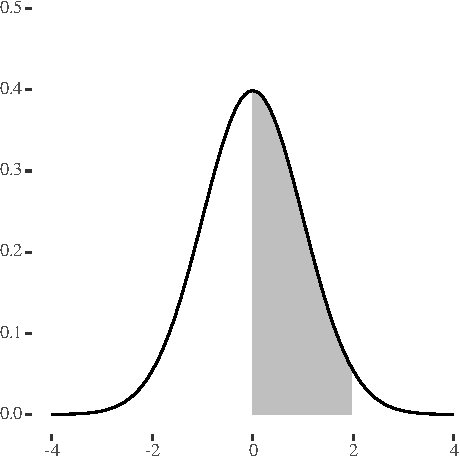
\includegraphics[width=0.8\linewidth]{DegreeOfFreedum_files/figure-latex/unnamed-chunk-1-1} 

}

\caption[母集団の分布]{母集団の分布}\label{fig:unnamed-chunk-1}
\end{figure}

\newpage

\hypertarget{ux7c21ux5358ux306aux30b7ux30dfux30e5ux30ecux30fcux30b7ux30e7ux30f3}{%
\subsection{\texorpdfstring{\textbf{簡単なシミュレーション}}{簡単なシミュレーション}}\label{ux7c21ux5358ux306aux30b7ux30dfux30e5ux30ecux30fcux30b7ux30e7ux30f3}}

 上記の母集団(\(x\))から以下の手順で二種類の変動(偏差平方和)を求めます。

\begin{enumerate}
\def\labelenumi{\arabic{enumi}.}
\tightlist
\item
  3つのデータをランダムサンプリングで取り出す(標本
  \(x_n, n = 1, 2, 3\))
\item
  取り出したデータの平均値(標本平均 \(\bar{x}\))を求める
\item
  標本平均(\(\bar{x}\))を用いて標本の変動(偏差平方和
  \(\sum_{i = 1}^{n}(x_i - \bar{x})^2\))を求める
\item
  母平均(\(\mu\))を用いて標本の変動(偏差平方和
  \(\sum_{i = 1}^{n}(x_i - \mu)^2\))を求める
\item
  求めた二つの変動(偏差平方和)を比較する
\end{enumerate}

この計算を任意の回数繰り返して標本平均(\(\bar{x}\))を用いた標本の変動(偏差平方和
\(\sum_{i = 1}^{n}(x_i - \bar{x})^2\))の方が小さいことを確認します。

\begin{Shaded}
\begin{Highlighting}[numbers=left,,]
\NormalTok{df }\OtherTok{\textless{}{-}} \FunctionTok{data.frame}\NormalTok{()}
\ControlFlowTok{for}\NormalTok{ (i }\ControlFlowTok{in} \FunctionTok{c}\NormalTok{(}\DecValTok{1}\SpecialCharTok{:}\DecValTok{30}\NormalTok{)) \{}
\NormalTok{  xs }\OtherTok{\textless{}{-}} \FunctionTok{sample}\NormalTok{(x, }\AttributeTok{size =} \DecValTok{3}\NormalTok{, }\AttributeTok{replace =} \ConstantTok{FALSE}\NormalTok{)  }\CommentTok{\# 母集団から3つのデータを取り出す}
\NormalTok{  xb }\OtherTok{\textless{}{-}} \FunctionTok{mean}\NormalTok{(xs)                  }\CommentTok{\# 標本平均を求める}
\NormalTok{  dssxb }\OtherTok{\textless{}{-}} \FunctionTok{sum}\NormalTok{((xs }\SpecialCharTok{{-}}\NormalTok{ xb)}\SpecialCharTok{\^{}}\DecValTok{2}\NormalTok{)       }\CommentTok{\# 標本平均を用いた変動(偏差平方和)}
\NormalTok{  dssmu }\OtherTok{\textless{}{-}} \FunctionTok{sum}\NormalTok{((xs }\SpecialCharTok{{-}}\NormalTok{ mu)}\SpecialCharTok{\^{}}\DecValTok{2}\NormalTok{)       }\CommentTok{\# 母平均を用いた変動(偏差平方和)}
  \CommentTok{\# 計算結果をデータフレームにまとめる}
\NormalTok{  dftmp }\OtherTok{\textless{}{-}} \FunctionTok{data.frame}\NormalTok{(}\AttributeTok{no =}\NormalTok{ i,     }\CommentTok{\# 通し番号}
                      \AttributeTok{x1 =}\NormalTok{ xs[}\DecValTok{1}\NormalTok{], }\CommentTok{\# 標本データ(n = 1)}
                      \AttributeTok{x2 =}\NormalTok{ xs[}\DecValTok{2}\NormalTok{], }\CommentTok{\# 標本データ(n = 2)}
                      \AttributeTok{x3 =}\NormalTok{ xs[}\DecValTok{3}\NormalTok{], }\CommentTok{\# 標本データ(n = 3)}
\NormalTok{                      xb,         }\CommentTok{\# 標本平均}
\NormalTok{                      mu,         }\CommentTok{\# 母平均}
\NormalTok{                      dssxb,      }\CommentTok{\# 標本平均を用いた変動(偏差平方和)}
\NormalTok{                      dssmu,      }\CommentTok{\# 母平均を用いた変動(偏差平方和)}
                      \AttributeTok{diff =}\NormalTok{ dssxb }\SpecialCharTok{{-}}\NormalTok{ dssmu  }\CommentTok{\# 負値なら標本平均による変動が小さい}
\NormalTok{                      )}
\NormalTok{  df }\OtherTok{\textless{}{-}}\NormalTok{ dplyr}\SpecialCharTok{::}\FunctionTok{bind\_rows}\NormalTok{(df, dftmp)}
\NormalTok{\}}

\NormalTok{df }\SpecialCharTok{\%\textgreater{}\%} 
\NormalTok{  dplyr}\SpecialCharTok{::}\FunctionTok{rename}\NormalTok{(}\StringTok{\textasciigrave{}}\AttributeTok{標本平均}\StringTok{\textasciigrave{}}\OtherTok{=}\NormalTok{ xb, }\StringTok{\textasciigrave{}}\AttributeTok{母平均}\StringTok{\textasciigrave{}} \OtherTok{=}\NormalTok{ mu,}
                \StringTok{\textasciigrave{}}\AttributeTok{標本平均での変動}\StringTok{\textasciigrave{}} \OtherTok{=}\NormalTok{ dssxb, }\StringTok{\textasciigrave{}}\AttributeTok{母平均での変動}\StringTok{\textasciigrave{}} \OtherTok{=}\NormalTok{ dssmu,}
                \StringTok{\textasciigrave{}}\AttributeTok{変動差(標本{-}母)}\StringTok{\textasciigrave{}} \OtherTok{=}\NormalTok{ diff) }\SpecialCharTok{\%\textgreater{}\%} 
  \FunctionTok{df\_print}\NormalTok{(}\AttributeTok{all =} \ConstantTok{TRUE}\NormalTok{, }\AttributeTok{scale\_down =} \ConstantTok{TRUE}\NormalTok{, }\AttributeTok{caption =} \StringTok{"シミュレーション結果"}\NormalTok{)}
\end{Highlighting}
\end{Shaded}

\begin{table}

\caption{\label{tab:unnamed-chunk-2}シミュレーション結果}
\centering
\resizebox{\linewidth}{!}{
\begin{tabular}[t]{rrrrrrrrr}
\toprule
no & x1 & x2 & x3 & 標本平均 & 母平均 & 標本平均での変動 & 母平均での変動 & 変動差(標本-母)\\
\midrule
\cellcolor{gray!6}{1} & \cellcolor{gray!6}{2.006349} & \cellcolor{gray!6}{4.9218712} & \cellcolor{gray!6}{13.662108} & \cellcolor{gray!6}{6.8634430} & \cellcolor{gray!6}{3.996745} & \cellcolor{gray!6}{73.5829117} & \cellcolor{gray!6}{98.236793} & \cellcolor{gray!6}{-24.6538812}\\
2 & 1.788097 & 0.3882464 & 9.061179 & 3.7458409 & 3.996745 & 43.3590209 & 43.547879 & -0.1888578\\
\cellcolor{gray!6}{3} & \cellcolor{gray!6}{4.911329} & \cellcolor{gray!6}{1.6467477} & \cellcolor{gray!6}{4.132243} & \cellcolor{gray!6}{3.5634399} & \cellcolor{gray!6}{3.996745} & \cellcolor{gray!6}{5.8140515} & \cellcolor{gray!6}{6.377310} & \cellcolor{gray!6}{-0.5632586}\\
4 & 7.012622 & 2.3197320 & 5.685805 & 5.0060530 & 3.996745 & 11.7047028 & 14.760814 & -3.0561109\\
\cellcolor{gray!6}{5} & \cellcolor{gray!6}{5.387746} & \cellcolor{gray!6}{3.5307648} & \cellcolor{gray!6}{5.427929} & \cellcolor{gray!6}{4.7821466} & \cellcolor{gray!6}{3.996745} & \cellcolor{gray!6}{2.3497420} & \cellcolor{gray!6}{4.200311} & \cellcolor{gray!6}{-1.8505694}\\
\addlinespace
6 & 2.101703 & 5.9993869 & 3.536314 & 3.8791345 & 3.996745 & 7.7722602 & 7.813756 & -0.0414963\\
\cellcolor{gray!6}{7} & \cellcolor{gray!6}{6.205521} & \cellcolor{gray!6}{4.1200703} & \cellcolor{gray!6}{4.464700} & \cellcolor{gray!6}{4.9300970} & \cellcolor{gray!6}{3.996745} & \cellcolor{gray!6}{2.4994440} & \cellcolor{gray!6}{5.112885} & \cellcolor{gray!6}{-2.6134408}\\
8 & 1.739977 & -3.7108190 & 9.146871 & 2.3920096 & 3.996745 & 83.2978089 & 91.023331 & -7.7255225\\
\cellcolor{gray!6}{9} & \cellcolor{gray!6}{4.071693} & \cellcolor{gray!6}{0.7495883} & \cellcolor{gray!6}{1.788127} & \cellcolor{gray!6}{2.2031361} & \cellcolor{gray!6}{3.996745} & \cellcolor{gray!6}{5.7765378} & \cellcolor{gray!6}{15.427630} & \cellcolor{gray!6}{-9.6510926}\\
10 & 5.066624 & 4.3646527 & 5.665752 & 5.0323429 & 3.996745 & 0.8481924 & 4.065585 & -3.2173922\\
\addlinespace
\cellcolor{gray!6}{11} & \cellcolor{gray!6}{3.162586} & \cellcolor{gray!6}{2.4739477} & \cellcolor{gray!6}{3.156060} & \cellcolor{gray!6}{2.9308644} & \cellcolor{gray!6}{3.996745} & \cellcolor{gray!6}{0.3131807} & \cellcolor{gray!6}{3.721481} & \cellcolor{gray!6}{-3.4083007}\\
12 & 3.426702 & 4.7470220 & 7.605623 & 5.2597821 & 3.996745 & 9.1260758 & 13.911868 & -4.7857920\\
\cellcolor{gray!6}{13} & \cellcolor{gray!6}{4.858415} & \cellcolor{gray!6}{6.6613752} & \cellcolor{gray!6}{3.807375} & \cellcolor{gray!6}{5.1090549} & \cellcolor{gray!6}{3.996745} & \cellcolor{gray!6}{4.1668899} & \cellcolor{gray!6}{7.878594} & \cellcolor{gray!6}{-3.7117037}\\
14 & 7.448547 & 7.1965942 & 0.596943 & 5.0806946 & 3.996745 & 30.1877836 & 33.712628 & -3.5248440\\
\cellcolor{gray!6}{15} & \cellcolor{gray!6}{5.204287} & \cellcolor{gray!6}{-4.9059256} & \cellcolor{gray!6}{1.280274} & \cellcolor{gray!6}{0.5262118} & \cellcolor{gray!6}{3.996745} & \cellcolor{gray!6}{51.9611147} & \cellcolor{gray!6}{88.094905} & \cellcolor{gray!6}{-36.1337908}\\
\addlinespace
16 & 2.670844 & 5.5704882 & 8.045905 & 5.4290791 & 3.996745 & 14.4756391 & 20.630386 & -6.1547472\\
\cellcolor{gray!6}{17} & \cellcolor{gray!6}{3.156763} & \cellcolor{gray!6}{-0.3528402} & \cellcolor{gray!6}{7.303819} & \cellcolor{gray!6}{3.3692471} & \cellcolor{gray!6}{3.996745} & \cellcolor{gray!6}{29.3799398} & \cellcolor{gray!6}{30.561199} & \cellcolor{gray!6}{-1.1812588}\\
18 & 4.551711 & 1.5130258 & 3.577730 & 3.2141556 & 3.996745 & 4.8150824 & 6.652418 & -1.8373358\\
\cellcolor{gray!6}{19} & \cellcolor{gray!6}{8.398765} & \cellcolor{gray!6}{7.4489186} & \cellcolor{gray!6}{3.508472} & \cellcolor{gray!6}{6.4520516} & \cellcolor{gray!6}{3.996745} & \cellcolor{gray!6}{13.4480976} & \cellcolor{gray!6}{31.533696} & \cellcolor{gray!6}{-18.0855988}\\
20 & 5.417183 & 5.9783885 & 5.468162 & 5.6212443 & 3.996745 & 0.1926273 & 8.109627 & -7.9169993\\
\addlinespace
\cellcolor{gray!6}{21} & \cellcolor{gray!6}{2.735636} & \cellcolor{gray!6}{7.3445911} & \cellcolor{gray!6}{5.119664} & \cellcolor{gray!6}{5.0666305} & \cellcolor{gray!6}{3.996745} & \cellcolor{gray!6}{10.6254527} & \cellcolor{gray!6}{14.059421} & \cellcolor{gray!6}{-3.4339684}\\
22 & 4.938459 & 4.7899228 & 1.256361 & 3.6615810 & 3.996745 & 8.6886552 & 9.025659 & -0.3370036\\
\cellcolor{gray!6}{23} & \cellcolor{gray!6}{1.475681} & \cellcolor{gray!6}{1.8195438} & \cellcolor{gray!6}{2.536436} & \cellcolor{gray!6}{1.9438869} & \cellcolor{gray!6}{3.996745} & \cellcolor{gray!6}{0.5857917} & \cellcolor{gray!6}{13.228464} & \cellcolor{gray!6}{-12.6426723}\\
24 & 8.819532 & 0.2646054 & 6.147329 & 5.0771555 & 3.996745 & 38.3112911 & 41.813155 & -3.5018640\\
\cellcolor{gray!6}{25} & \cellcolor{gray!6}{4.115611} & \cellcolor{gray!6}{5.3069370} & \cellcolor{gray!6}{4.355087} & \cellcolor{gray!6}{4.5925452} & \cellcolor{gray!6}{3.996745} & \cellcolor{gray!6}{0.7942081} & \cellcolor{gray!6}{1.859144} & \cellcolor{gray!6}{-1.0649354}\\
\addlinespace
26 & 4.166215 & 4.7324917 & 2.513740 & 3.8041492 & 3.996745 & 2.6580668 & 2.769346 & -0.1112788\\
\cellcolor{gray!6}{27} & \cellcolor{gray!6}{2.464780} & \cellcolor{gray!6}{6.2689757} & \cellcolor{gray!6}{1.749776} & \cellcolor{gray!6}{3.4945107} & \cellcolor{gray!6}{3.996745} & \cellcolor{gray!6}{11.8020997} & \cellcolor{gray!6}{12.558816} & \cellcolor{gray!6}{-0.7567164}\\
28 & 7.425591 & 2.2166859 & 4.767910 & 4.8033957 & 3.996745 & 13.5682362 & 15.520295 & -1.9520586\\
\cellcolor{gray!6}{29} & \cellcolor{gray!6}{3.258395} & \cellcolor{gray!6}{6.3141248} & \cellcolor{gray!6}{4.093102} & \cellcolor{gray!6}{4.5552074} & \cellcolor{gray!6}{3.996745} & \cellcolor{gray!6}{4.9890542} & \cellcolor{gray!6}{5.924697} & \cellcolor{gray!6}{-0.9356424}\\
30 & 5.353118 & 1.2392623 & 4.160559 & 3.5843131 & 3.996745 & 8.9599938 & 9.470293 & -0.5102988\\
\bottomrule
\end{tabular}}
\end{table}

\begin{figure}

{\centering 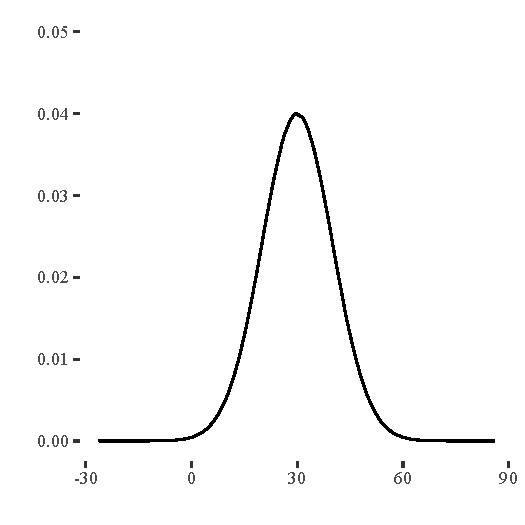
\includegraphics[width=0.8\linewidth]{DegreeOfFreedum_files/figure-latex/unnamed-chunk-3-1} 

}

\caption[標本平均を用いた変動と母平均を用いた変動の差]{標本平均を用いた変動と母平均を用いた変動の差}\label{fig:unnamed-chunk-3}
\end{figure}

\newpage

\hypertarget{ux6a19ux672cux6a19ux6e96ux504fux5deeux306eux88dcux6b63ux5024ux3092ux78baux8a8dux3059ux308b}{%
\section{\texorpdfstring{\textbf{標本標準偏差の補正値を確認する}}{標本標準偏差の補正値を確認する}}\label{ux6a19ux672cux6a19ux6e96ux504fux5deeux306eux88dcux6b63ux5024ux3092ux78baux8a8dux3059ux308b}}

 標本平均(\(\bar{x}\))を用いた変動(偏差平方和)は母平均(\(\mu\))を用いた変動(偏差平方和)よりも小さくなることがわかりました。では、自由度で補正した標準偏差が母標準偏差に本当に近くなるのかを同じ母集団(\(x\))を使って確認します。

\begin{Shaded}
\begin{Highlighting}[numbers=left,,]
\NormalTok{df }\OtherTok{\textless{}{-}} \FunctionTok{data.frame}\NormalTok{()}
\NormalTok{m }\OtherTok{\textless{}{-}} \DecValTok{12}
\ControlFlowTok{for}\NormalTok{ (i }\ControlFlowTok{in} \FunctionTok{c}\NormalTok{(}\DecValTok{1}\SpecialCharTok{:}\DecValTok{30}\NormalTok{)) \{}
\NormalTok{  xs }\OtherTok{\textless{}{-}} \FunctionTok{sample}\NormalTok{(x, }\AttributeTok{size =}\NormalTok{ m, }\AttributeTok{replace =} \ConstantTok{FALSE}\NormalTok{)  }\CommentTok{\# 母集団から3つのデータを取り出す}
\NormalTok{  xb }\OtherTok{\textless{}{-}} \FunctionTok{mean}\NormalTok{(xs)                              }\CommentTok{\# 標本平均を求める}
\NormalTok{  sdxb }\OtherTok{\textless{}{-}} \FunctionTok{sqrt}\NormalTok{(}\FunctionTok{sum}\NormalTok{((xs }\SpecialCharTok{{-}}\NormalTok{ xb)}\SpecialCharTok{\^{}}\DecValTok{2}\NormalTok{) }\SpecialCharTok{/}\NormalTok{ (m }\SpecialCharTok{{-}} \DecValTok{1}\NormalTok{))    }\CommentTok{\# 自由度で補正した標本標準偏差}
\NormalTok{  sdmu }\OtherTok{\textless{}{-}} \FunctionTok{sqrt}\NormalTok{(}\FunctionTok{sum}\NormalTok{((xs }\SpecialCharTok{{-}}\NormalTok{ mu)}\SpecialCharTok{\^{}}\DecValTok{2}\NormalTok{) }\SpecialCharTok{/}\NormalTok{ m)          }\CommentTok{\# 母標準偏差}
  \CommentTok{\# 計算結果をデータフレームにまとめる}
\NormalTok{  dftmp }\OtherTok{\textless{}{-}} \FunctionTok{data.frame}\NormalTok{(}\AttributeTok{no =}\NormalTok{ i,             }\CommentTok{\# 通し番号}
                      \AttributeTok{x1 =}\NormalTok{ xs[}\DecValTok{1}\NormalTok{],         }\CommentTok{\# 標本データ(n = 1)}
                      \AttributeTok{x2 =}\NormalTok{ xs[}\DecValTok{2}\NormalTok{],         }\CommentTok{\# 標本データ(n = 2)}
                      \AttributeTok{x3 =}\NormalTok{ xs[}\DecValTok{3}\NormalTok{],         }\CommentTok{\# 標本データ(n = 3)}
\NormalTok{                      xb,                 }\CommentTok{\# 標本平均}
\NormalTok{                      mu,                 }\CommentTok{\# 母平均}
\NormalTok{                      sdxb,               }\CommentTok{\# 補正した標本標準偏差(不偏推定値)}
\NormalTok{                      sdmu,               }\CommentTok{\# 母標準偏差}
                      \AttributeTok{diff =}\NormalTok{ sdxb }\SpecialCharTok{{-}}\NormalTok{ sdmu  }\CommentTok{\# 負値なら標本平均による変動が小さい}
\NormalTok{                      )}
\NormalTok{  df }\OtherTok{\textless{}{-}}\NormalTok{ dplyr}\SpecialCharTok{::}\FunctionTok{bind\_rows}\NormalTok{(df, dftmp)}
\NormalTok{\}}

\NormalTok{df }\SpecialCharTok{\%\textgreater{}\%} 
\NormalTok{  dplyr}\SpecialCharTok{::}\FunctionTok{rename}\NormalTok{(}\StringTok{\textasciigrave{}}\AttributeTok{標本平均}\StringTok{\textasciigrave{}}\OtherTok{=}\NormalTok{ xb, }\StringTok{\textasciigrave{}}\AttributeTok{母平均}\StringTok{\textasciigrave{}} \OtherTok{=}\NormalTok{ mu,}
                \StringTok{\textasciigrave{}}\AttributeTok{補正した標本標準偏差}\StringTok{\textasciigrave{}} \OtherTok{=}\NormalTok{ sdxb, }\StringTok{\textasciigrave{}}\AttributeTok{母標準偏差}\StringTok{\textasciigrave{}} \OtherTok{=}\NormalTok{ sdmu,}
                \StringTok{\textasciigrave{}}\AttributeTok{差(標本{-}母)}\StringTok{\textasciigrave{}} \OtherTok{=}\NormalTok{ diff) }\SpecialCharTok{\%\textgreater{}\%} 
  \FunctionTok{df\_print}\NormalTok{(}\AttributeTok{all =} \ConstantTok{TRUE}\NormalTok{, }\AttributeTok{scale\_down =} \ConstantTok{TRUE}\NormalTok{, }\AttributeTok{caption =} \StringTok{"シミュレーション結果"}\NormalTok{)}
\end{Highlighting}
\end{Shaded}

\begin{table}

\caption{\label{tab:unnamed-chunk-4}シミュレーション結果}
\centering
\resizebox{\linewidth}{!}{
\begin{tabular}[t]{rrrrrrrrr}
\toprule
no & x1 & x2 & x3 & 標本平均 & 母平均 & 補正した標本標準偏差 & 母標準偏差 & 差(標本-母)\\
\midrule
\cellcolor{gray!6}{1} & \cellcolor{gray!6}{5.9005759} & \cellcolor{gray!6}{7.1291092} & \cellcolor{gray!6}{3.8242538} & \cellcolor{gray!6}{3.614148} & \cellcolor{gray!6}{3.996745} & \cellcolor{gray!6}{2.586970} & \cellcolor{gray!6}{2.506211} & \cellcolor{gray!6}{0.0807592}\\
2 & 6.0248282 & 5.8620663 & 2.2198528 & 4.603901 & 3.996745 & 2.607905 & 2.569638 & 0.0382661\\
\cellcolor{gray!6}{3} & \cellcolor{gray!6}{6.4648030} & \cellcolor{gray!6}{3.5847104} & \cellcolor{gray!6}{2.5342685} & \cellcolor{gray!6}{5.089606} & \cellcolor{gray!6}{3.996745} & \cellcolor{gray!6}{2.494076} & \cellcolor{gray!6}{2.626098} & \cellcolor{gray!6}{-0.1320228}\\
4 & -0.8838906 & 4.3998278 & 1.7926698 & 4.800031 & 3.996745 & 3.038578 & 3.018081 & 0.0204970\\
\cellcolor{gray!6}{5} & \cellcolor{gray!6}{-4.5942678} & \cellcolor{gray!6}{1.0893745} & \cellcolor{gray!6}{0.4178212} & \cellcolor{gray!6}{2.565047} & \cellcolor{gray!6}{3.996745} & \cellcolor{gray!6}{3.663974} & \cellcolor{gray!6}{3.788897} & \cellcolor{gray!6}{-0.1249226}\\
\addlinespace
6 & 5.3967884 & 3.8588633 & 2.1832539 & 4.261000 & 3.996745 & 2.706099 & 2.604334 & 0.1017651\\
\cellcolor{gray!6}{7} & \cellcolor{gray!6}{6.8730200} & \cellcolor{gray!6}{7.2502373} & \cellcolor{gray!6}{5.6432586} & \cellcolor{gray!6}{5.456434} & \cellcolor{gray!6}{3.996745} & \cellcolor{gray!6}{3.830144} & \cellcolor{gray!6}{3.946922} & \cellcolor{gray!6}{-0.1167784}\\
8 & 0.5408073 & 4.6170769 & 5.8160347 & 3.987181 & 3.996745 & 2.642547 & 2.530064 & 0.1124828\\
\cellcolor{gray!6}{9} & \cellcolor{gray!6}{-0.1232023} & \cellcolor{gray!6}{1.7702919} & \cellcolor{gray!6}{2.8303924} & \cellcolor{gray!6}{2.410388} & \cellcolor{gray!6}{3.996745} & \cellcolor{gray!6}{2.112865} & \cellcolor{gray!6}{2.570741} & \cellcolor{gray!6}{-0.4578755}\\
10 & 3.0938152 & 3.4629398 & 6.1279842 & 3.502391 & 3.996745 & 2.252870 & 2.212884 & 0.0399858\\
\addlinespace
\cellcolor{gray!6}{11} & \cellcolor{gray!6}{4.3994310} & \cellcolor{gray!6}{7.0916869} & \cellcolor{gray!6}{3.1375773} & \cellcolor{gray!6}{3.809455} & \cellcolor{gray!6}{3.996745} & \cellcolor{gray!6}{2.191099} & \cellcolor{gray!6}{2.106162} & \cellcolor{gray!6}{0.0849376}\\
12 & 6.2870186 & 9.1389105 & 0.0862662 & 4.409378 & 3.996745 & 2.810322 & 2.722135 & 0.0881873\\
\cellcolor{gray!6}{13} & \cellcolor{gray!6}{6.8602403} & \cellcolor{gray!6}{10.4291384} & \cellcolor{gray!6}{9.6602453} & \cellcolor{gray!6}{4.463471} & \cellcolor{gray!6}{3.996745} & \cellcolor{gray!6}{3.401384} & \cellcolor{gray!6}{3.289852} & \cellcolor{gray!6}{0.1115316}\\
14 & 9.6864373 & 2.1238370 & 1.2698589 & 4.606710 & 3.996745 & 3.791487 & 3.680963 & 0.1105247\\
\cellcolor{gray!6}{15} & \cellcolor{gray!6}{6.3649314} & \cellcolor{gray!6}{0.9749754} & \cellcolor{gray!6}{3.4152821} & \cellcolor{gray!6}{4.939895} & \cellcolor{gray!6}{3.996745} & \cellcolor{gray!6}{2.568665} & \cellcolor{gray!6}{2.633958} & \cellcolor{gray!6}{-0.0652933}\\
\addlinespace
16 & 0.3682559 & 2.8779801 & 5.5504674 & 4.240597 & 3.996745 & 4.441971 & 4.259849 & 0.1821222\\
\cellcolor{gray!6}{17} & \cellcolor{gray!6}{5.8434016} & \cellcolor{gray!6}{5.2180801} & \cellcolor{gray!6}{1.6120696} & \cellcolor{gray!6}{4.306186} & \cellcolor{gray!6}{3.996745} & \cellcolor{gray!6}{2.870485} & \cellcolor{gray!6}{2.765646} & \cellcolor{gray!6}{0.1048390}\\
18 & 4.5487401 & 0.9673316 & 6.2789387 & 2.854302 & 3.996745 & 2.001293 & 2.230826 & -0.2295327\\
\cellcolor{gray!6}{19} & \cellcolor{gray!6}{3.6510340} & \cellcolor{gray!6}{5.0247488} & \cellcolor{gray!6}{2.7621445} & \cellcolor{gray!6}{3.788562} & \cellcolor{gray!6}{3.996745} & \cellcolor{gray!6}{1.957817} & \cellcolor{gray!6}{1.885993} & \cellcolor{gray!6}{0.0718247}\\
20 & 5.6092354 & 7.7755369 & 2.8950185 & 5.226601 & 3.996745 & 2.121617 & 2.374595 & -0.2529779\\
\addlinespace
\cellcolor{gray!6}{21} & \cellcolor{gray!6}{6.2705511} & \cellcolor{gray!6}{8.0279919} & \cellcolor{gray!6}{0.4769332} & \cellcolor{gray!6}{4.696590} & \cellcolor{gray!6}{3.996745} & \cellcolor{gray!6}{3.965896} & \cellcolor{gray!6}{3.861013} & \cellcolor{gray!6}{0.1048832}\\
22 & -3.1034010 & 2.6415654 & 5.6015774 & 1.792153 & 3.996745 & 3.843142 & 4.289423 & -0.4462814\\
\cellcolor{gray!6}{23} & \cellcolor{gray!6}{1.9884340} & \cellcolor{gray!6}{1.4358724} & \cellcolor{gray!6}{4.4602812} & \cellcolor{gray!6}{3.354269} & \cellcolor{gray!6}{3.996745} & \cellcolor{gray!6}{1.940232} & \cellcolor{gray!6}{1.965596} & \cellcolor{gray!6}{-0.0253637}\\
24 & 2.2377706 & 2.9119022 & -0.9604801 & 2.612762 & 3.996745 & 2.432963 & 2.709509 & -0.2765463\\
\cellcolor{gray!6}{25} & \cellcolor{gray!6}{10.1334809} & \cellcolor{gray!6}{9.3962861} & \cellcolor{gray!6}{0.9661430} & \cellcolor{gray!6}{4.402635} & \cellcolor{gray!6}{3.996745} & \cellcolor{gray!6}{3.630622} & \cellcolor{gray!6}{3.499673} & \cellcolor{gray!6}{0.1309489}\\
\addlinespace
26 & 1.4913636 & 2.2132959 & 3.8690116 & 3.775323 & 3.996745 & 2.509745 & 2.413078 & 0.0966669\\
\cellcolor{gray!6}{27} & \cellcolor{gray!6}{0.6061874} & \cellcolor{gray!6}{5.7470604} & \cellcolor{gray!6}{6.8969015} & \cellcolor{gray!6}{3.734887} & \cellcolor{gray!6}{3.996745} & \cellcolor{gray!6}{2.320765} & \cellcolor{gray!6}{2.237340} & \cellcolor{gray!6}{0.0834250}\\
28 & 0.7757434 & 4.4510336 & 6.5881741 & 4.846286 & 3.996745 & 2.941545 & 2.941657 & -0.0001128\\
\cellcolor{gray!6}{29} & \cellcolor{gray!6}{4.1562629} & \cellcolor{gray!6}{-0.1827302} & \cellcolor{gray!6}{4.1072400} & \cellcolor{gray!6}{3.105353} & \cellcolor{gray!6}{3.996745} & \cellcolor{gray!6}{2.683109} & \cellcolor{gray!6}{2.719142} & \cellcolor{gray!6}{-0.0360325}\\
30 & 5.7547576 & 4.5193953 & 6.3142889 & 3.847106 & 3.996745 & 3.060298 & 2.933831 & 0.1264671\\
\bottomrule
\end{tabular}}
\end{table}

\begin{figure}

{\centering 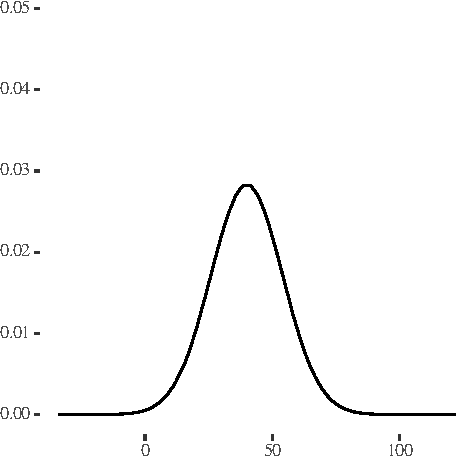
\includegraphics[width=0.8\linewidth]{DegreeOfFreedum_files/figure-latex/unnamed-chunk-5-1} 

}

\caption[標本標準偏差の補正値(不偏推定値)と母標準偏差の差]{標本標準偏差の補正値(不偏推定値)と母標準偏差の差}\label{fig:unnamed-chunk-5}
\end{figure}

\newpage

\hypertarget{ux304aux308fux308aux306b}{%
\section{\texorpdfstring{\textbf{おわりに}}{おわりに}}\label{ux304aux308fux308aux306b}}

 詳細で理論的な説明が必要な場合は『なぜ不偏分散は N-1
で割るのか』\citep{estpdf82:online}を参照してください。

ちなみに母集団(\(x\))の平均値(\(mu\))と標準偏差(\(s\))は以下の通りでした。

\begin{Shaded}
\begin{Highlighting}[numbers=left,,]
\FunctionTok{mean}\NormalTok{(x)                }\CommentTok{\# 平均値}
\end{Highlighting}
\end{Shaded}

\begin{verbatim}
## [1] 3.996744
\end{verbatim}

\begin{Shaded}
\begin{Highlighting}[numbers=left,,]
\NormalTok{(n }\SpecialCharTok{/}\NormalTok{ (n }\SpecialCharTok{{-}} \DecValTok{1}\NormalTok{)) }\SpecialCharTok{*} \FunctionTok{sd}\NormalTok{(x)  }\CommentTok{\# 標準偏差}
\end{Highlighting}
\end{Shaded}

\begin{verbatim}
## [1] 2.992983
\end{verbatim}

 

\bibliography{bib/references.bib}



\end{document}
